\documentclass{beamer}
\usetheme{tokitex}

\usepackage{tikz}
\usepackage{graphics}
\usepackage{multirow}
\usepackage{tabto}
\usepackage{xspace}
\usepackage{amsmath}

\usepackage{tikz}
\usepackage{clrscode3e}

\usepackage[english,bahasa]{babel}
\newtranslation[to=bahasa]{Section}{Bagian}
\newtranslation[to=bahasa]{Subsection}{Subbagian}

\usepackage{listings, lstautogobble}
\usepackage{color}

\definecolor{dkgreen}{rgb}{0,0.6,0}
\definecolor{gray}{rgb}{0.5,0.5,0.5}
\definecolor{mauve}{rgb}{0.58,0,0.82}

\lstset{frame=tb,
  language=pascal,
  aboveskip=1mm,
  belowskip=1mm,
  showstringspaces=false,
  columns=fullflexible,
  keepspaces=true,
  basicstyle={\small\ttfamily},
  numbers=none,
  numberstyle=\tiny\color{gray},
  keywordstyle=\color{blue},
  commentstyle=\color{dkgreen},
  stringstyle=\color{mauve},
  breaklines=true,
  breakatwhitespace=true,
  autogobble=true
}

\usepackage{caption}
\captionsetup[figure]{labelformat=empty}

\newcommand{\progTerm}[1]{\textbf{#1}}
\newcommand{\foreignTerm}[1]{\textit{#1}}
\newcommand{\newTerm}[1]{\alert{\textbf{#1}}}
\newcommand{\emp}[1]{\alert{#1}}
\newcommand{\statement}[1]{"#1"}

% Getting tired of writing \foreignTerm all the time
\newcommand{\farray}{\foreignTerm{array}\xspace}
\newcommand{\fArray}{\foreignTerm{Array}\xspace}
\newcommand{\foverhead}{\foreignTerm{overhead}\xspace}
\newcommand{\fOverhead}{\foreignTerm{Overhead}\xspace}
\newcommand{\fsubarray}{\foreignTerm{subarray}\xspace}
\newcommand{\fSubarray}{\foreignTerm{Subarray}\xspace}
\newcommand{\fbasecase}{\foreignTerm{base case}\xspace}
\newcommand{\fBasecase}{\foreignTerm{Base case}\xspace}
\newcommand{\ftopdown}{\foreignTerm{top down}\xspace}
\newcommand{\fTopdown}{\foreignTerm{Top down}\xspace}
\newcommand{\fbottomup}{\foreignTerm{bottom up}\xspace}
\newcommand{\fBottomup}{\foreignTerm{Bottom up}\xspace}
\newcommand{\fpruning}{\foreignTerm{pruning}\xspace}
\newcommand{\fPruning}{\foreignTerm{Pruning}\xspace}

\newcommand{\fgraph}{\foreignTerm{graph}\xspace}
\newcommand{\fGraph}{\foreignTerm{Graph}\xspace}
\newcommand{\fnode}{\foreignTerm{node}\xspace}
\newcommand{\fNode}{\foreignTerm{Node}\xspace}
\newcommand{\fedge}{\foreignTerm{edge}\xspace}
\newcommand{\fEdge}{\foreignTerm{Edge}\xspace}
\newcommand{\fdegree}{\foreignTerm{degree}\xspace}
\newcommand{\fDegree}{\foreignTerm{Degree}\xspace}
\newcommand{\fadjacencylist}{\foreignTerm{adjacency list}\xspace}
\newcommand{\fAdjacencylist}{\foreignTerm{Adjacency list}\xspace}
\newcommand{\fadjacencymatrix}{\foreignTerm{adjacency matrix}\xspace}
\newcommand{\fAdjacencymatrix}{\foreignTerm{Adjacency matrix}\xspace}
\newcommand{\fedgelist}{\foreignTerm{edge list}\xspace}
\newcommand{\fEdgelist}{\foreignTerm{Edge list}\xspace}
\newcommand{\flist}{\foreignTerm{list}\xspace}
\newcommand{\fList}{\foreignTerm{List}\xspace}
\newcommand{\fgraphtraversal}{\foreignTerm{graph traversal}\xspace}
\newcommand{\fGraphtraversal}{\foreignTerm{Graph traversal}\xspace}
\newcommand{\ftree}{\foreignTerm{tree}\xspace}
\newcommand{\fTree}{\foreignTerm{Tree}\xspace}

\newcommand{\fDivideAndConquer}{\foreignTerm{Divide and Conquer}\xspace}
\newcommand{\fMergeSort}{\foreignTerm{Merge Sort}\xspace}
\newcommand{\fQuickSort}{\foreignTerm{Quicksort}\xspace}
\newcommand{\fpivot}{\foreignTerm{pivot}\xspace}
\newcommand{\fPivot}{\foreignTerm{Pivot}\xspace}
\newcommand{\fBruteForce}{\foreignTerm{Brute Force}\xspace}
\newcommand{\fCompleteSearch}{\foreignTerm{Complete Search}\xspace}
\newcommand{\fExhaustiveSearch}{\foreignTerm{Exhaustive Search}\xspace}
\newcommand{\fBinarySearch}{\foreignTerm{Binary Search}\xspace}
\newcommand{\fGreedy}{\foreignTerm{Greedy}\xspace}
\newcommand{\fGreedyChoice}{\foreignTerm{Greedy Choice}\xspace}

\newcommand{\pheap}{\progTerm{heap}\xspace}
\newcommand{\pHeap}{\progTerm{Heap}\xspace}
\newcommand{\pBinaryHeap}{\progTerm{Binary Heap}\xspace}
\newcommand{\pbinaryHeap}{\progTerm{binary heap}\xspace}

\title{Struktur Data Non Linear: \newline Heap}
\author{Tim Olimpiade Komputer Indonesia}
\date{}

\begin{document}

\begin{frame}
\titlepage
\end{frame}

\begin{frame}
\frametitle{Pendahuluan}
Melalui dokumen ini, kalian akan:
\begin{itemize}
  \item Mengenal dan mengimplementasikan struktur data \pheap.
  \item Mengetahui mengapa diperlukan \pheap.
\end{itemize}
\end{frame}

\begin{frame}
\frametitle{Motivasi}
Anda diberikan sejumlah operasi. Setiap operasi dapat berbentuk salah satu dari:
\begin{itemize}
  \item add($x$), artinya simpan bilangan $x$.
  \item getMax(), artinya  dapatkan bilangan terbesar yang saat ini masih disimpan.
  \item deleteMax(), artinya  hapus bilangan terbesar dari penyimpanan.
\end{itemize}
\end{frame}

\begin{frame}
\frametitle{Motivasi}
Berikut contoh operasinya dan perilaku yang diharapkan:
\begin{itemize}
  \item add(5), bilangan yang disimpan: [5].
  \item add(7), bilangan yang disimpan: [5, 7].
  \item add(3), bilangan yang disimpan: [5, 7, 3].
  \item getMax(), laporkan bahwa 7 merupakan bilangan terbesar.
  \item deleteMax(), bilangan yang disimpan: [5, 3].
  \item getMax(), laporkan bahwa 5 merupakan bilangan terbesar.
\end{itemize}
\end{frame}

\begin{frame}
\frametitle{Solusi Sederhana}
\begin{itemize}
  \item Solusi paling mudah adalah membuat sebuah \farray besar dan variabel yang menunjukkan posisi terakhir elemen pada \farray.
  \item Untuk setiap operasi add($x$), tambahkan elemen \farray, geser variabel penunjuk, lalu urutkan data. 
  \item Operasi getMax() dapat dilayani dengan mengembalikan elemen terbesar.
  \item Operasi deleteMax() dapat dilayani dengan menggeser variabel penunjuk.
\end{itemize}
\end{frame}

\begin{frame}
\frametitle{Analisis Solusi Sederhana}
\begin{itemize}
  \item Misalkan $N$ menyatakan banyaknya elemen pada \farray.
  \item Dengan cara ini, operasi add($x$) berlangsung dalam $O(N \log{N})$, apabila pengurutannya menggunakan \progTerm{Quicksort}.
  \item Operasi getMax() dan deleteMax() berlangsung dalam $O(1)$.
  \newline
  \item Perhatikan bahwa pengurutan akan lebih efisien jika digunakan \progTerm{Insertion Sort}, sehingga kompleksitas add($x$) menjadi $O(N)$.
\end{itemize}
\end{frame}

\begin{frame}
\frametitle{Analisis Solusi Sederhana}
\begin{table}[ht]
  \begin{tabular}{|l|c|}
    \hline Operasi  & Dengan Sorting\\
    \hline  add($x$) & $O(N)$  \\
    \hline  getMax() & $O(1)$ \\
    \hline  deleteMax() & $O(1)$ \\
    \hline
  \end{tabular}
\end{table}  
\end{frame}

\begin{frame}
\frametitle{Masalah Solusi Sederhana}
\begin{itemize}
  \item Solusi sederhana ini tidak efisien ketika banyak dilakukan operasi add($x$).
  \item Kita akan mempelajari bagaimana \pheap mengatasi masalah ini secara efisien.
\end{itemize}
\end{frame}

\section{Pengenalan Heap}
\frame{\sectionpage}

\begin{frame}
\frametitle{Heap}
\begin{itemize}
  \item \pHeap merupakan struktur data yang umum dikenal pada ilmu komputer.
  \item Nama \pheap sendiri berasal dari Bahasa Inggris, yang berarti "gundukan". 
\end{itemize}
\end{frame}

\begin{frame}
\frametitle{Operasi Heap}
\pHeap mendukung operasi:
\begin{itemize}
  \item \progTerm{Push}, yaitu memasukan elemen baru ke penyimpanan.
  \item \progTerm{Pop}, yaitu membuang elemen \textbf{terbesar} dari penyimpanan.
  \item \progTerm{Top}, yaitu mengakses elemen \textbf{terbesar} dari penyimpanan. 
\end{itemize}
\end{frame}

\begin{frame}
\frametitle{Cara Kerja Heap}
\begin{itemize}
  \item \pHeap dapat diimplementasikan dengan berbagai cara.
  \item Kita akan mempelajari salah satunya, yaitu \pBinaryHeap.
  \item Sebelum itu, diperlukan pengetahuan mengenai \progTerm{tree}.
\end{itemize}
\end{frame}

\begin{frame}
\frametitle{Tree}
\begin{itemize}
  \item Seperti yang telah dipelajari, \ftree merupakan suatu \fgraph yang setiap \fnode-nya saling terhubung dan tidak memiliki \foreignTerm{cycle}.
\end{itemize}
\begin{figure}
  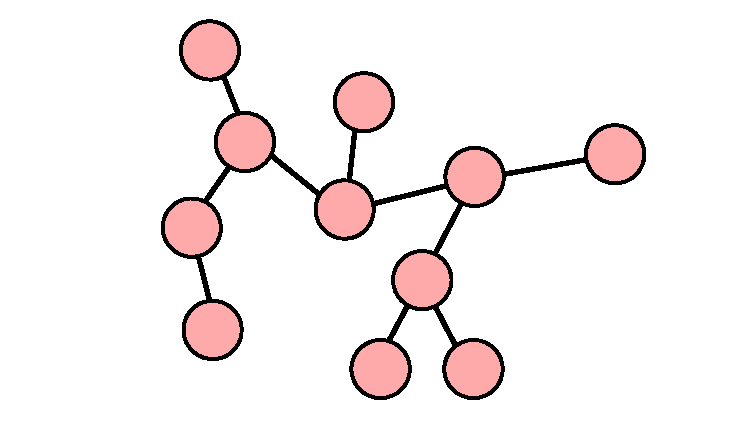
\includegraphics[width=7cm]{asset/tree.pdf}
\end{figure}
\end{frame}

\begin{frame}
\frametitle{Rooted Tree}
\begin{itemize}
  \item Suatu \ftree yang memiliki akar, atau \fnode yang berada di paling atas disebut sebagai \foreignTerm{rooted-tree}.
\end{itemize}
\begin{figure}
  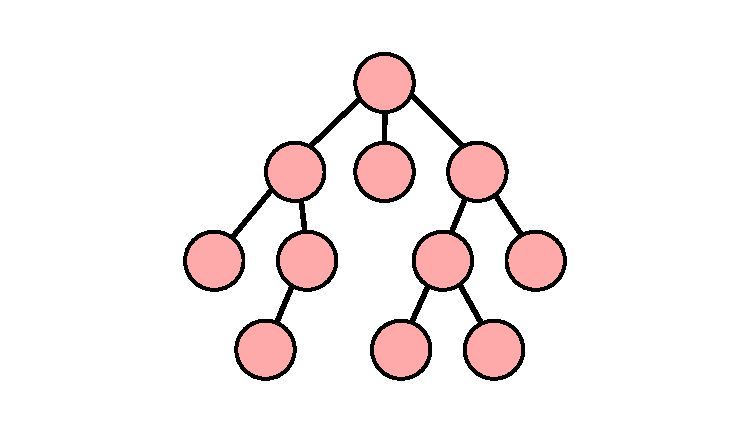
\includegraphics[width=7cm]{asset/rooted-tree.pdf}
\end{figure}
\end{frame}

\begin{frame}
\frametitle{Binary Tree}
\begin{itemize}
  \item Suatu \foreignTerm{rooted-tree} yang setiap \fnode-nya memiliki 0, 1, atau 2 anak disebut dengan \foreignTerm{Binary Tree}.
\end{itemize}
\begin{figure}
  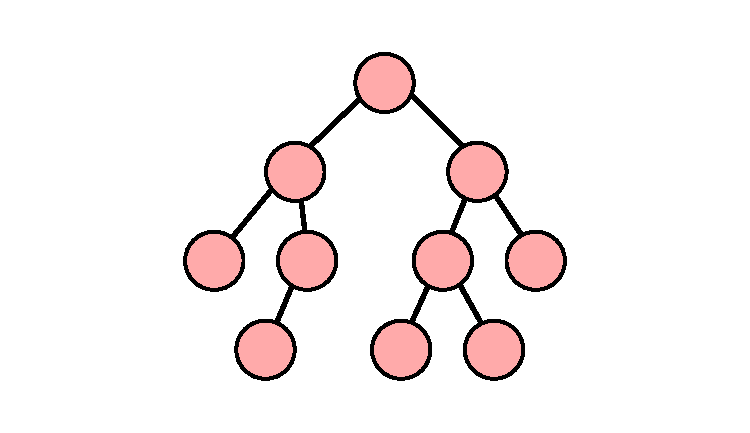
\includegraphics[width=7cm]{asset/binary-tree.pdf}
\end{figure}
\end{frame}

\begin{frame}
\frametitle{Full Binary Tree}
\begin{itemize}
  \item Suatu \foreignTerm{binary tree} yang seluruh \fnode-nya memiliki 2 anak, kecuali tingkat paling bawah yang tidak memiliki anak, disebut dengan \foreignTerm{Full Binary Tree}
  \item Bila banyaknya \fnode adalah $N$, maka ketinggiannya adalah $O(\log{N})$.
\end{itemize}
\begin{figure}
  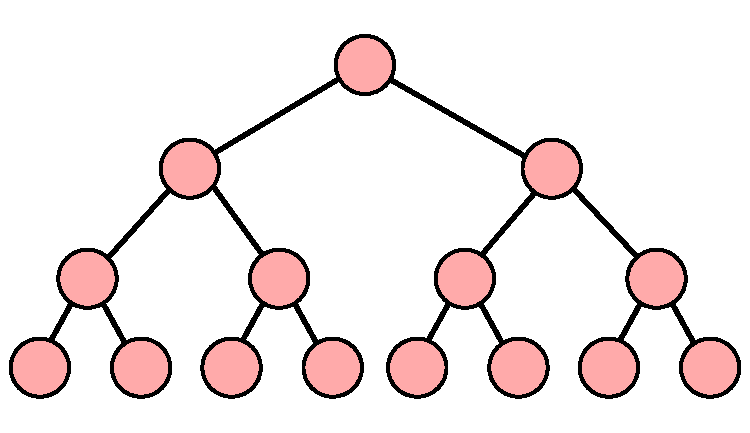
\includegraphics[width=7cm]{asset/full-binary-tree.pdf}
\end{figure}
\end{frame}

\begin{frame}
\frametitle{Complete Binary Tree}
\foreignTerm{Complete Binary Tree} adalah \foreignTerm{binary tree} yang:
\begin{itemize}
  \item Seluruh \fnode-nya memiliki 2 anak, kecuali tingkat paling bawah.
  \item Tingkat paling bawahnya dapat terisi sebagian, tetapi harus terisi dari kiri ke kanan.
\end{itemize}
\begin{figure}
  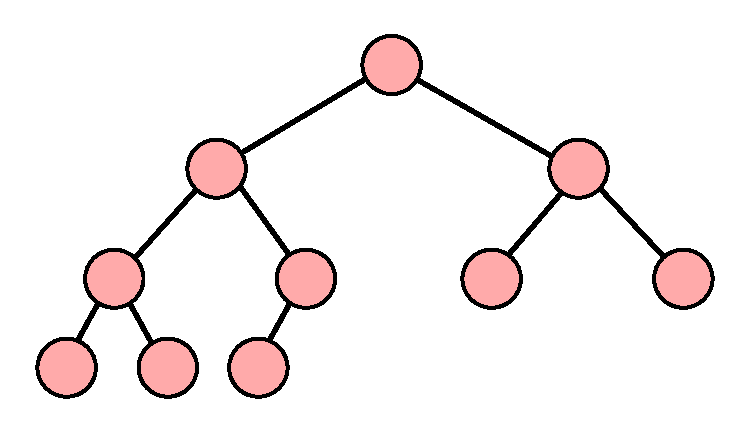
\includegraphics[width=7cm]{asset/complete-binary-tree.pdf}
\end{figure}
\begin{itemize}
  \item Bila banyaknya \fnode adalah $N$, maka ketinggiannya \\ adalah $O(\log{N})$.
\end{itemize}
\end{frame}

\begin{frame}
\frametitle{Bukan Complete Binary Tree}
Berikut bukan \foreignTerm{Complete Binary Tree}, sebab elemen di tingkat paling bawah tidak berisi dari kiri ke kanan (terdapat lubang).
\begin{figure}
  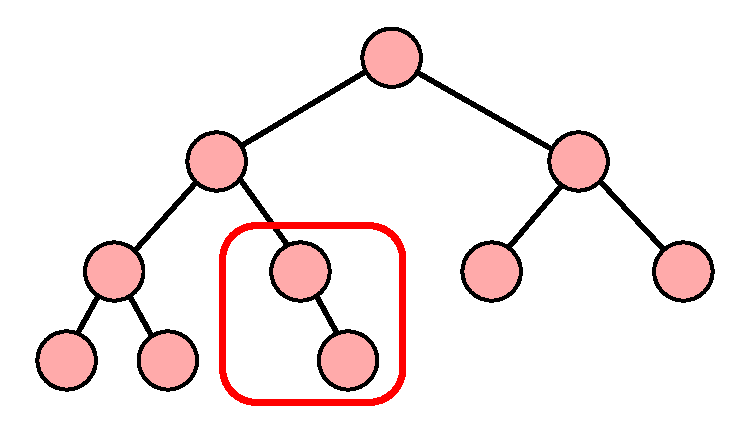
\includegraphics[width=7cm]{asset/not-complete-binary-tree-1.pdf}
\end{figure}
\end{frame}

\begin{frame}
\frametitle{Bukan Complete Binary Tree}
Berikut juga bukan \foreignTerm{Complete Binary Tree}, sebab terdapat \fnode tanpa 2 anak pada tingkat bukan paling bawah.
\begin{figure}
  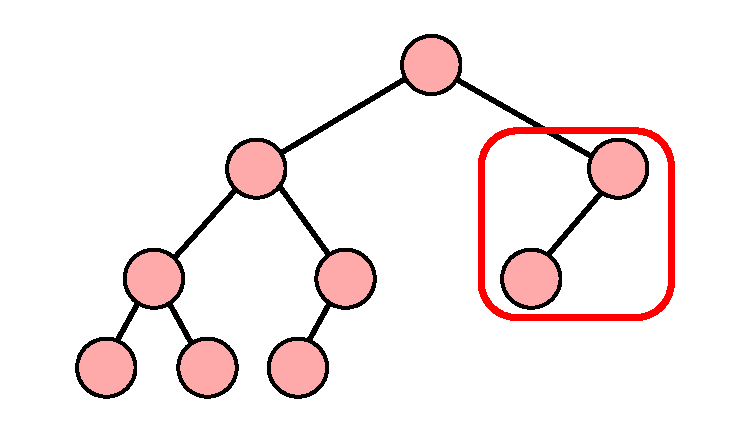
\includegraphics[width=7cm]{asset/not-complete-binary-tree-2.pdf}
\end{figure}
\end{frame}

\begin{frame}
\frametitle{Struktur Binary Heap}
Struktur data \pbinaryHeap memiliki sifat:
\begin{itemize}
  \item Berstruktur \foreignTerm{complete binary tree}.
  \item Setiap \fnode merepresentasikan elemen yang disimpan pada \pheap.
  \item Setiap \fnode memiliki nilai yang \textbf{lebih besar} daripada \fnode anak-anaknya.
\end{itemize}
\end{frame}

\begin{frame}
\frametitle{Contoh Binary Heap}
\begin{figure}
  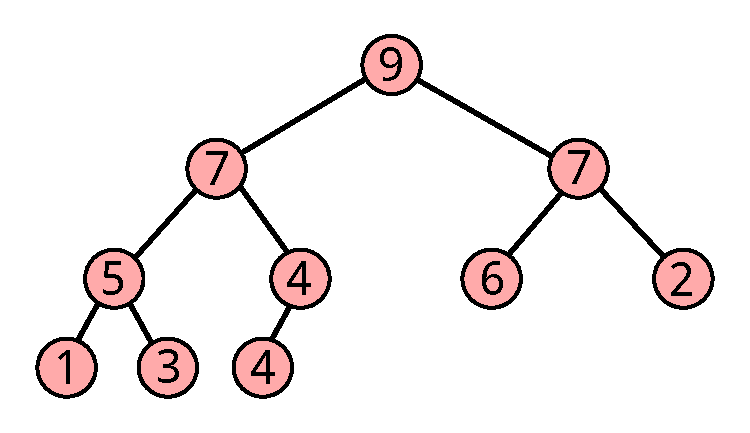
\includegraphics[width=9cm]{asset/heap.pdf}
\end{figure}
\end{frame}

\begin{frame}
\frametitle{Contoh Bukan Binary Heap}
Bukan binary heap.
\begin{figure}
  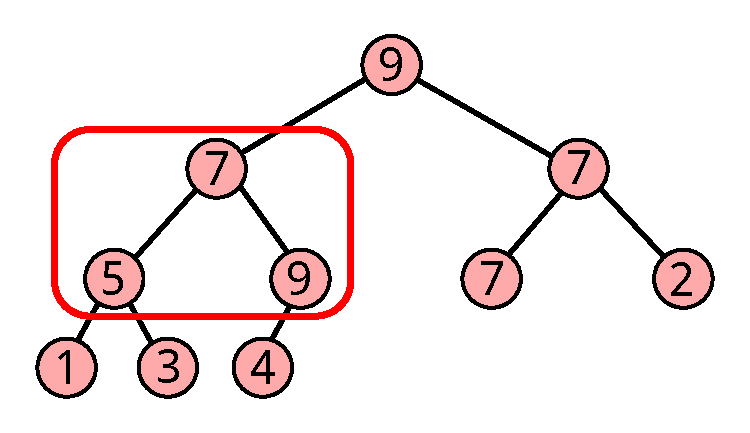
\includegraphics[width=9cm]{asset/not-heap.pdf}
\end{figure}
\end{frame}

\begin{frame}
\frametitle{Mengapa Harus Demikian?}
\begin{itemize}
  \item Struktur seperti ini menjamin operasi-operasi yang dilayani \pheap dapat dilakukan secara efisien.
  \item Misalkan $N$ adalah banyaknya elemen yang sedang disimpan.
  \item Operasi \progTerm{push} dan \progTerm{pop} bekerja dalam $O(\log{N})$, sementara \progTerm{top} bekerja dalam $O(1)$.
  \item Kita akan melihat satu per satu bagaimana operasi tersebut dilaksanakan.
\end{itemize}
\end{frame}

\begin{frame}
\frametitle{Operasi Push}
Melakukan \foreignTerm{push} pada \pbinaryHeap dilakukan dengan 2 tahap:
\begin{itemize}
  \item Tambahkan \fnode baru di posisi yang memenuhi aturan \foreignTerm{complete binary tree}.
  \item Selama elemen \fnode yang merupakan orang tua langsung dari elemen ini memiliki nilai yang lebih kecil, tukar nilai elemen kedua \fnode tersebut.
\end{itemize}
\end{frame}

\begin{frame}
\frametitle{Operasi Push}
Sebagai contoh, misalkan hendak ditambahkan elemen bernilai 8 ke suatu \pbinaryHeap berikut:
\begin{figure}
  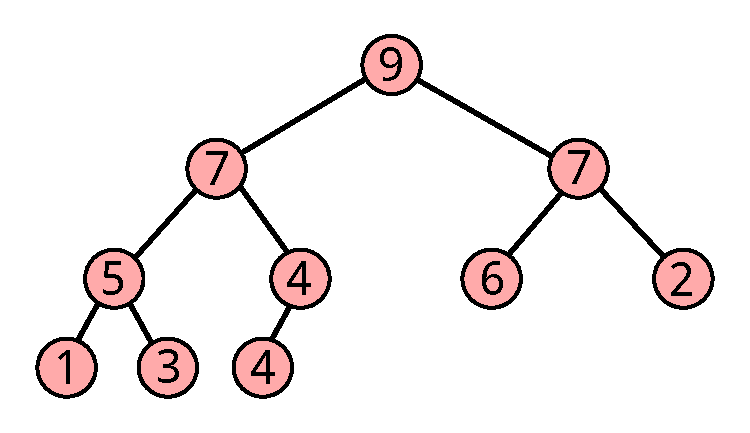
\includegraphics[width=9cm]{asset/heap.pdf}
\end{figure}
\end{frame}

\begin{frame}
\frametitle{Operasi Push (lanj.)}
Tambahkan \fnode.
\begin{figure}
  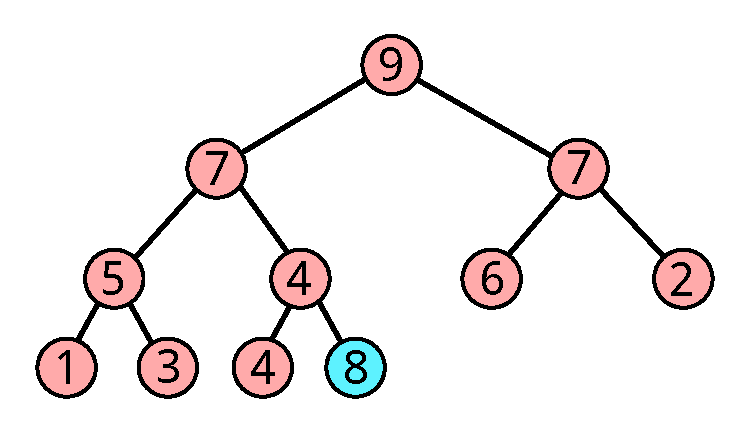
\includegraphics[width=9cm]{asset/push-1.pdf}
\end{figure}
\end{frame}

\begin{frame}
\frametitle{Operasi Push (lanj.)}
Karena orang tua-nya memiliki nilai lebih kecil, tukar nilainya.
\begin{figure}
  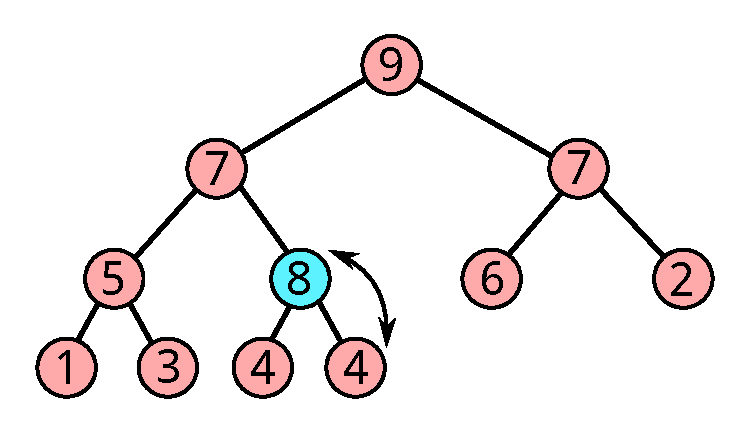
\includegraphics[width=9cm]{asset/push-2.pdf}
\end{figure}
\end{frame}

\begin{frame}
\frametitle{Operasi Push (lanj.)}
Karena orang tua-nya masih memiliki nilai lebih kecil, tukar lagi.
\begin{figure}
  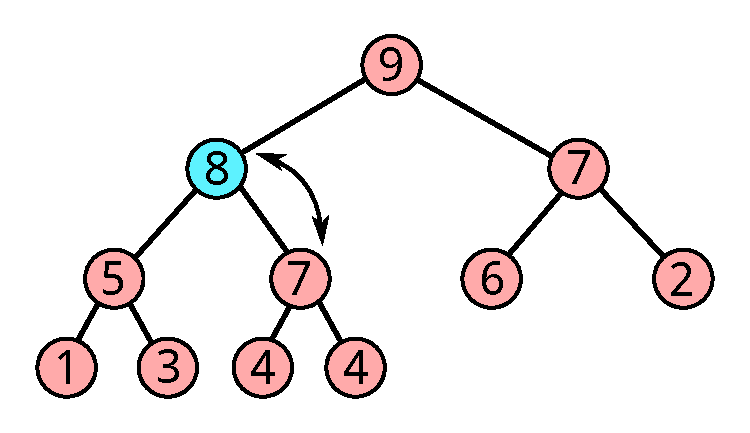
\includegraphics[width=9cm]{asset/push-3.pdf}
\end{figure}
\end{frame}

\begin{frame}
\frametitle{Operasi Push (lanj.)}
Orang tua-nya sudah memiliki nilai yang lebih besar.\newline Operasi push selesai.
\begin{figure}
  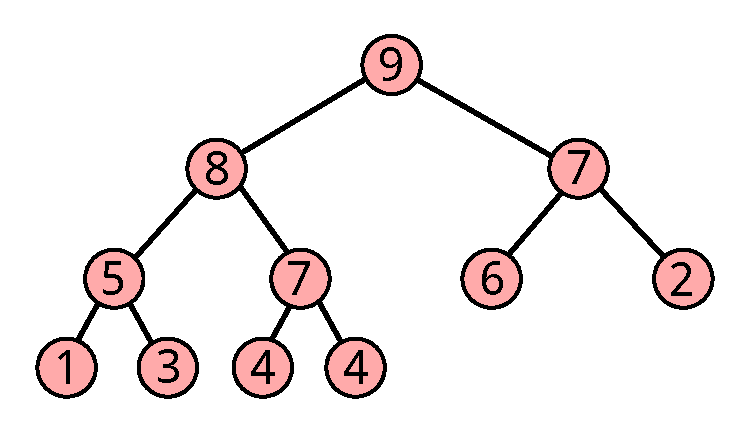
\includegraphics[width=9cm]{asset/push-4.pdf}
\end{figure}
\end{frame}

\begin{frame}
\frametitle{Kompleksitas Push}
\begin{itemize}
  \item Kasus terburuk terjadi ketika pertukaran yang terjadi paling banyak.
  \item Hal ini terjadi ketika elemen yang dimasukkan merupakan nilai yang paling besar pada \pheap.
  \item Banyaknya pertukaran yang terjadi sebanding dengan kedalaman dari \foreignTerm{compete binary tree}.
  \item Kompleksitas untuk operasi \foreignTerm{push} adalah $O(\log{N})$.
\end{itemize}
\end{frame}

\begin{frame}
\frametitle{Operasi Pop}
Melakukan \foreignTerm{pop} pada \pbinaryHeap dilakukan dengan 2 tahap:
\begin{itemize}
  \item Tukar posisi elemen pada \foreignTerm{root} dengan elemen terakhir mengikuti aturan \foreignTerm{complete binary tree}.
  \item Buang elemen terakhir \pbinaryHeap, yang telah berisi elemen dari \foreignTerm{root}.
  \item Selama elemen yang ditukar ke posisi \foreignTerm{root} memiliki anak langsung yang berelemen lebih besar, tukar elemen tersebut dengan salah anaknya yang memiliki elemen \textbf{terbesar}. 
\end{itemize}
\end{frame}

\begin{frame}
\frametitle{Operasi Pop (lanj.)}
Misalkan akan dilakukan pop pada \pheap berikut:
\begin{figure}
  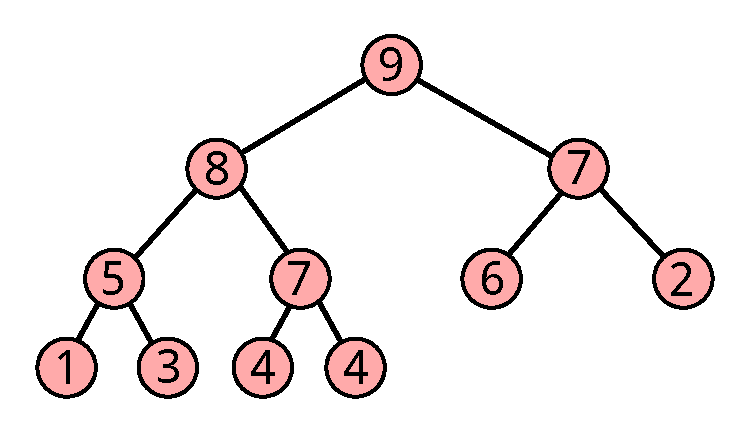
\includegraphics[width=9cm]{asset/pop-1.pdf}
\end{figure}
\end{frame}

\begin{frame}
\frametitle{Operasi Pop (lanj.)}
Tukar elemen pada \foreignTerm{root} dengan elemen terakhir pada \foreignTerm{complete binary tree}.
\begin{figure}
  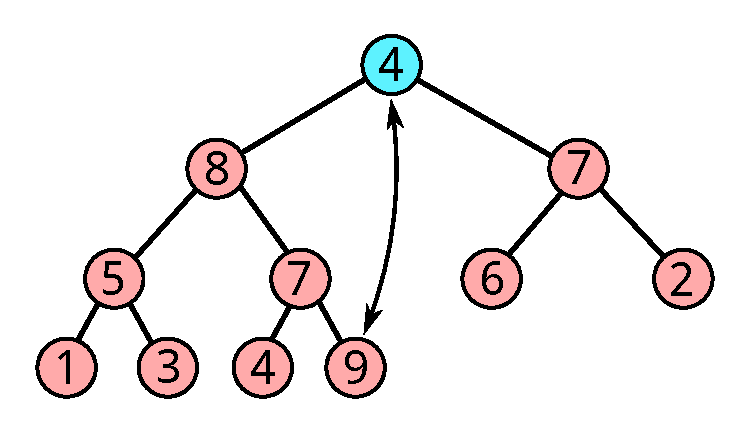
\includegraphics[width=9cm]{asset/pop-2.pdf}
\end{figure}
\end{frame}

\begin{frame}
\frametitle{Operasi Pop (lanj.)}
Buang elemen terakhir.
\begin{figure}
  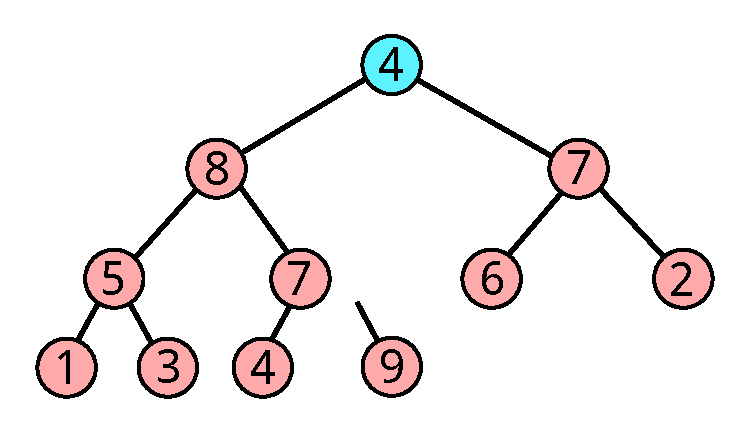
\includegraphics[width=9cm]{asset/pop-3.pdf}
\end{figure}
\end{frame}

\begin{frame}
\frametitle{Operasi Pop (lanj.)}
Perbaiki struktur \pheap dengan menukar elemen pada \foreignTerm{root} dengan anaknya yang bernilai \textbf{terbesar}.
\begin{figure}
  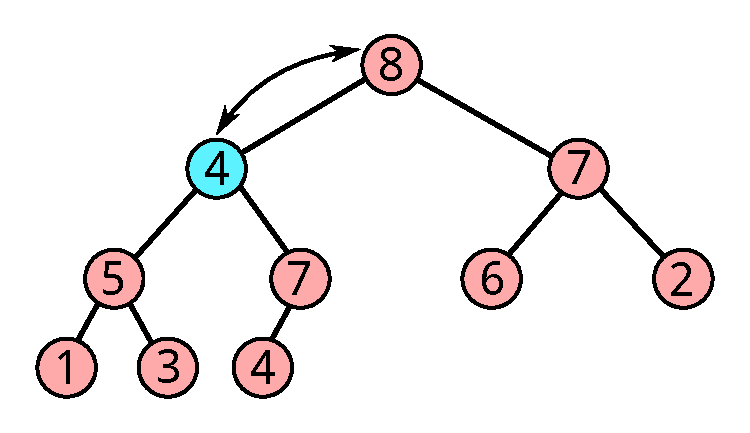
\includegraphics[width=9cm]{asset/pop-4.pdf}
\end{figure}
\end{frame}

\begin{frame}
\frametitle{Operasi Pop (lanj.)}
Karena masih terdapat anaknya yang lebih besar, tukar lagi.
\begin{figure}
  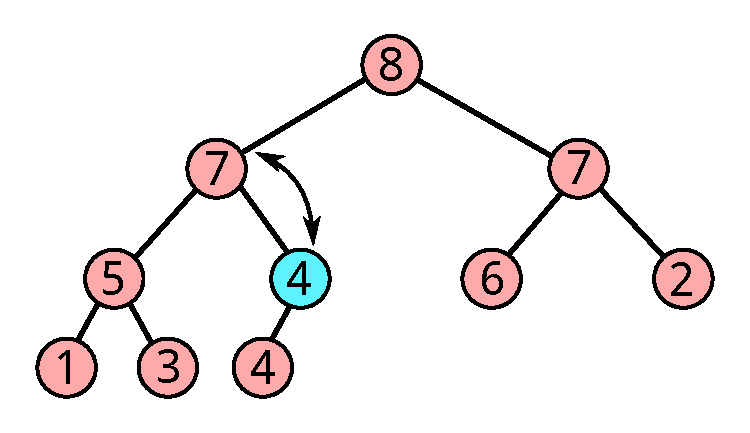
\includegraphics[width=9cm]{asset/pop-5.pdf}
\end{figure}
\end{frame}

\begin{frame}
\frametitle{Operasi Pop (lanj.)}
Kini sudah tidak ada anak yang bernilai lebih besar, operasi pop selesai.
\begin{figure}
  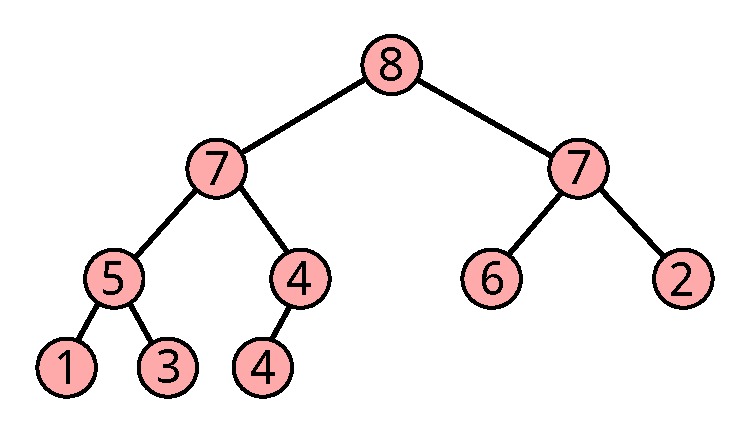
\includegraphics[width=9cm]{asset/pop-6.pdf}
\end{figure}
\end{frame}

\begin{frame}
\frametitle{Kompleksitas Pop}
\begin{itemize}
  \item Kasus terburuk juga terjadi ketika pertukaran yang terjadi paling banyak.
  \item Hal ini terjadi ketika elemen yang ditempatkan di \foreignTerm{root} cukup kecil, sehingga perlu ditukar sampai ke tingkat paling bawah.
  \item Banyaknya pertukaran yang terjadi sebanding dengan kedalaman dari \foreignTerm{compete binary tree}.
  \item Kompleksitas untuk operasi \foreignTerm{pop} adalah $O(\log{N})$.
\end{itemize}
\end{frame}

\begin{frame}
\frametitle{Operasi Top}
\begin{itemize}
  \item Operasi ini sebenarnya sesederhana mengembalikan elemen pada \foreignTerm{root} \pbinaryHeap.
  \item Kompleksitas operasi ini adalah $O(1)$.
\end{itemize}
\end{frame}

\begin{frame}
\frametitle{Analisis Solusi dengan Heap}
Penerapan \pheap pada persoalan motivasi:
\begin{table}[ht]
  \begin{tabular}{|l|c|c|}
    \hline Operasi  & Dengan Sorting & Dengan Heap \\
    \hline  add($x$) & $O(N)$ & $O(\log{N})$\\
    \hline  getMax() & $O(1)$ & $O(1)$\\
    \hline  deleteMax() & $O(1)$ & $O(\log{N})$\\
    \hline
  \end{tabular}
\end{table}  

Kini seluruh operasi dapat dilakukan dengan efisien.
\end{frame}

\section{Implementasi Binary Heap}
\frame{\sectionpage}

\begin{frame}
\frametitle{Membuat Tree}
\begin{itemize}
  \item Representasi \ftree pada implementasi dapat menggunakan teknik representasi \fgraph yang telah dipelajari sebelumnya.
  \item Namun, untuk \ftree dengan kondisi tertentu, kita dapat menggunakan representasi yang lebih sederhana.
  \item Terutama pada kasus ini, yang mana \ftree yang diperlukan adalah \foreignTerm{complete binary tree}.
\end{itemize}
\end{frame}

\begin{frame}
\frametitle{Representasi Complete Binary Tree}
\begin{itemize}
  \item Kedengarannya kurang masuk akal, tetapi \foreignTerm{complete binary tree} dapat direpresentasikan dengan sebuah \farray.
  \item Misalkan \farray ini bersifat \foreignTerm{zero-based}, yaitu dimulai dari indeks 0.
  \item Elemen pada indeks ke-$i$ menyatakan elemen pada \fnode ke-$i$.
  \item Anak kiri dari \fnode ke-$i$ adalah \fnode ke-$(2i+1)$. 
  \item Anak kanan dari \fnode ke-$i$ adalah \fnode ke-$(2i+2)$. 
\end{itemize}
\end{frame}

\begin{frame}
\frametitle{Representasi Complete Binary Tree (lanj.)}
\begin{figure}
  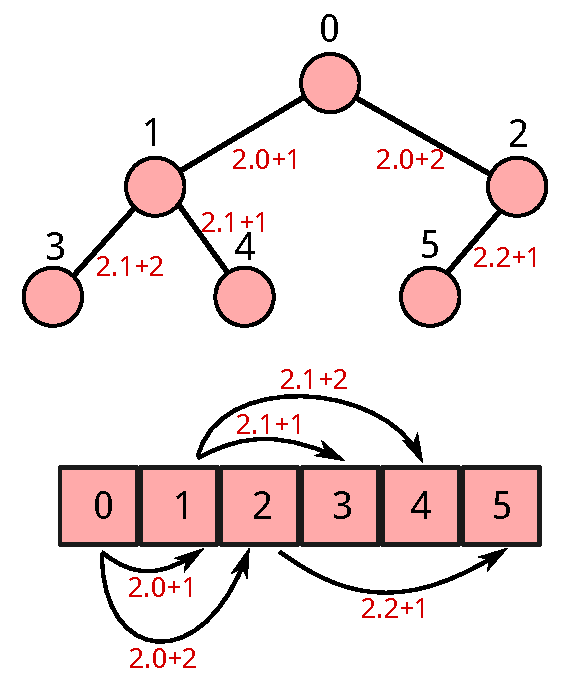
\includegraphics[width=6cm]{asset/heap-array.pdf}
\end{figure}
\end{frame}

\begin{frame}
\frametitle{Representasi Complete Binary Tree (lanj.)}
\begin{itemize}
  \item Dengan logika yang serupa, orang tua dari \fnode ke-$i$ adalah \fnode ke-$\lfloor\frac{i-1}{2}\rfloor$.
  \item Apabila Anda memutuskan untuk menggunakan \foreignTerm{one-based}, berarti rumusnya menjadi:
  \begin{itemize}
    \item Anak kiri: $2i$.
    \item Anak kanan: $2i+1$.
    \item Orang tua: $\lfloor \frac{i}{2} \rfloor$
  \end{itemize}
  \item Representasi ini sangat mempermudah implementasi \pbinaryHeap.
\end{itemize}
\end{frame}

\begin{frame}
\frametitle{Representasi Array}
\begin{itemize}
  \item Karena panjang \farray dapat bertambah atau berkurang, diperlukan \farray yang ukurannya dinamis.
  \item Pada contoh ini, kita akan menggunakan \farray berukuran statis dan sebuah variabel yang menyatakan ukuran \farray saat ini.
  \item Berikut prosedur untuk inisialisasi, dengan asumsi $maxSize$ menyatakan ukuran terbesar pada \pheap yang mungkin.
\end{itemize}
\begin{codebox}
\Procname{$\proc{initializeHeap}(maxSize)$}
\li \Comment Buat array $arr$ berukuran $maxSize$
\li $size \gets 0$
\end{codebox}
\end{frame}

\begin{frame}
\frametitle{Implementasi Fungsi Pembantu}
Buat juga beberapa fungsi yang akan membantu mempermudah penulisan kode.
\begin{codebox}
\Procname{$\proc{getParent}(x)$}
\li \Return $\proc{floor}((x-1) / 2)$
\end{codebox}

\begin{codebox}
\Procname{$\proc{getLeft}(x)$}
\li \Return $2x + 1$
\end{codebox}

\begin{codebox}
\Procname{$\proc{getRight}(x)$}
\li \Return $2x + 2$
\end{codebox}
\end{frame}

\begin{frame}
\frametitle{Implementasi Push}
\begin{codebox}
\Procname{$\proc{push}(val)$}
\li $i \gets size$
\li $arr[i] \gets val$
\li \While $(i > 0) \land (arr[i] > arr[\proc{getParent}(i)])$  \Do
\li   $\proc{swap}(arr[i], arr[\proc{getParent}(i)])$
\li   $i \gets \proc{getParent}(i)$
    \End
\li $size \gets size + 1$
\end{codebox}
\end{frame}

\begin{frame}
\frametitle{Implementasi Pop}
\begin{codebox}
\Procname{$\proc{pop}()$}
\li $swap(arr[0], arr[size-1])$
\li $i \gets 0$
\li $swapped \gets true$
\li \While $swapped$  \Do
\li   $maxIdx \gets i$
\li   \If $(\proc{getLeft}(i) < size) \land (arr[maxIdx] < arr[\proc{getLeft}(i)])$ \Then
\li     $maxIdx \gets \proc{getLeft}(i)$
      \End
\li   \If $(\proc{getRight}(i) < size) \land (arr[maxIdx] < arr[\proc{getRight}(i)])$ \Then
\li     $maxIdx \gets \proc{getRight}(i)$
      \End
\li   $\proc{swap}(arr[i], arr[maxIdx])$
\li   $swapped \gets (maxIdx \ne i)$ 
\Comment $true$ bila terjadi pertukaran
\li   $i = maxIdx$
    \End
\li $size \gets size - 1$
\end{codebox}
\end{frame}

\begin{frame}
\frametitle{Implementasi Top}
\begin{codebox}
\Procname{$\proc{top}()$}
\li \Return $arr[size-1]$
\end{codebox}

... sangat sederhana
\end{frame}

\begin{frame}
\frametitle{Catatan Implementasi}
\begin{itemize}
  \item Tentu saja, Anda dapat membuat \pheap dengan urutan yang terbalik, yaitu elemen terkecilnya di atas.
  \item Dengan demikian, operasi yang didukung adalah mencari atau menghapus elemen terkecil.
  \item Biasanya \pheap dengan sifat ini disebut dengan \progTerm{min-heap}, sementara \pheap dengan elemen terbesar di atas disebut dengan \progTerm{max-heap}.
\end{itemize}
\end{frame}

\begin{frame}
\frametitle{Manfaat Heap}
\begin{itemize}
  \item Pada ilmu komputer, \pheap dapat digunakan sebagai \textit{priority queue}, yaitu antrian yang terurut menurut suatu kriteria.
  \item Sifat \pheap juga dapat digunakan untuk optimisasi suatu algoritma. Contoh paling nyatanya adalah untuk mempercepat algoritma \progTerm{Dijkstra}.
  \item Berbagai solusi persoalan \progTerm{greedy} juga dapat diimplementasikan secara efisien dengan \pheap.
\end{itemize}
\end{frame}

\begin{frame}
\frametitle{Library Heap}
\begin{itemize}
  \item Bagi pengguna C++, struktur data "priority\_queue" dari include algorithm merupakan struktur data \pheap.
  \item Bagi pengguna Pascal, Anda perlu mengimplementasikan \pheap sendiri.
\end{itemize}
\end{frame}

\begin{frame}
\frametitle{Penutup}
\begin{itemize}
  \item Dengan mempelajari \pheap, Anda memperdalam pemahaman tentang bagaimana penggunaan struktur data yang tepat dapat membantu menyelesaikan persoalan tertentu.
  \item Terdapat bagian yang tidak dibahas pada tulisan ini, yaitu tentang pembuatan \pheap dari sebuah \farray berisi $N$ bilangan dalam $O(N)$.
  \item Pembaca yang tertarik dapat membaca lebih lanjut pada \href{https://en.wikipedia.org/wiki/Heap\_\%28data\_structure\%29}{\underline{tulisan berikut}}.
\end{itemize}
\end{frame}

\end{document}


